\section{Introduction}\label{s:intro}

This paper introduces the idea of {\em site-to-site} Internet traffic control. By ``site'', we mean a single physical location with tens to many thousands of endpoints sharing access links to rest of the Internet. Examples of sites include a company office, a coworking office building, a university campus, a single datacenter, and a point-of-presence (PoP) of a regional Internet Service Provider (ISP). 

%When a site originates traffic, the administrator of the site often has high-level objectives for their traffic, but cannot achieve those objectives today because the bottlenecks are elsewhere. 

Consider a company site with employees running thousands of concurrent applications. The administrator may wish to enforce certain traffic control policies for the company; for example, ensuring rates and priorities for Zoom sessions, de-prioritizing bulk backup traffic, prioritizing interactive web sessions, and so on. There are two issues that stand in the way: first, the bottleneck for these traffic flows may not be in the company's network, and second, the applications could all be transiting different bottlenecks. So what is the company to do?
%, and experiencing poor quality because of traffic from other sources outside the company's control. 

Cloud computing has made the second issue manageable. Because the cloud has become the prevalent method to deploy applications today, applications from different vendors often run from a small number of cloud sites (e.g., Amazon, Azure, etc.). This means that the network path used by these multiple applications serving the company's users are likely to share a common bottleneck; for example, all the applications running from Amazon's US-West datacenter, all the video sessions from a given Zoom datacenter, and so on. In this setting,  by treating the traffic between the datacenter site and the company site as a single aggregate, the company's network administrator may be able to achieve their traffic control objectives.

%e.g., ensuring that video sessions get adequate rates, de-prioritizing bulk backup traffic, prioritizing interactive web sessions, etc.

But what about the first issue? The bottleneck for all the traffic between Amazon US-West and the company may not be the site's access link or at Amazon, but elsewhere, e.g., within the company's ISP; indeed, that may be the common case~\cite{inferring-interdomain-congestion, isp-throttle-1, isp-throttle-2, isp-throttle-3}. Unfortunately, the company cannot control traffic when the queues are inside its ISP. And the ISP can't help because it does not know what the company's objectives are.\footnote{Interdomain QoS mechanisms~\cite{braden1997resource, wroclawski1997use} have not succeeded in the Internet despite years of effort.}

%a coworking space might want fairness between the traffic of resident companies to different cloud datacenters. A company may want to prioritize video conferencing traffic over other traffic (e.g., bulk backup). 

%% Example objectives

We propose a system, {\em \name}, that solves this problem. \name enables flexible control of a traffic {\em bundle} between a source site and a destination site by {\em shifting} the queues that would otherwise have accumulated elsewhere to the source's site (Figure~\ref{fig:design:shift-bottleneck}) \cut{\radhika{should we instead refer to Fig 2 here?}}. It then schedules packets from this shifted queue using standard techniques~\cite{diffserv, fair-queueing, sfq, pie, CoDel, fifoplus, virtualClocks, csfq, drr, red, ecn} to reduce mean flow-completion times, ensure low packet delays, isolate classes of traffic from each other, etc.

%The most effective place to enforce a scheduling policy is where queue buildup occurs; where there is queueing, there is the opportunity to reorder packets and apply mechanisms~\cite{diffserv, fair-queueing, sfq, pie, CoDel, fifoplus, virtualClocks, csfq, drr, red, ecn} to reduce mean flow-completion times, ensure low packet delays, isolate classes of traffic from each other, etc.

%An increasing number of use cases involve sites that need to exchange large quantities of traffic on the Internet. 
%Examples include traffic between a content provider (\eg Amazon, Google, etc.) and a network with many clients (\eg an enterprise), between two different campuses of an organization, between collaborating institutes, and so on.

%The flows within such a bundle are likely to share common bottlenecks in the network connecting the two domains (as shown in F). 
The key idea in \name is a control loop between the source and destination sites to calculate the dynamic rate for the bundle. Rather than terminate end-to-end connections at the sites, we leave them intact and develop an ``inner loop'' control method between the two sites that computes this rate. The inner control loop uses a delay-based congestion control algorithm that ensures high throughput, but controls {\em self-inflicted queueing delays} at the actual bottleneck. By avoiding queues at the bottleneck, the source site can prioritize latency-sensitive applications and allocate rates according to its objectives.

By not terminating the end-to-end connections at the sites, \name{} achieves a key benefit: if the bottleneck congestion is due to other traffic not from the bundle, end-to-end algorithms naturally find their fair-share. It also simplifies the implementation because \name{} does not have to proxy TCP, QUIC, and other end-to-end protocols.

%Bundler uses a middlebox at the source site and another at the destination site to determine the time-varying rate of the path between the sites using a control loop


%\an{maybe refer to figure 1/example scenario? or cite something? as is, this seems like a point reviewers might complain about.}

 %Such links with queue build-up are often outside the control of individual content providers, which prevents them from enjoying the benefits of scheduling.
%content providers and end users have been unable to enjoy the benefits of scheduling policies. 

% ISP's cant solve problem (e.g. with CSFQ)

\if 0
ISPs, on the other hand, do control the bottleneck links in their carrier networks where different scheduling and queue management policies can be effectively enforced. 
However, ISPs neither have enough visibility into their customers' traffic to choose desired policies on their queues, nor enough incentives to enforce them\footnote{The case for private WANs is different, since they are owned by a single entity, and have, thus, been successful in exploiting the benefits of scheduling~\cite{swan, b4, bwe}. Our focus is public networks.}. Even if an ISP isolates each its customers' traffic (\eg with fair queueing~\cite{fair-queueing}), that still does not serve a customer's desire to enforce different scheduling policies within its own traffic.  
Large customers might be able to negotiate expensive deals with certain carriers to enforce specific policies~\cite{att-qos}. 
However, it might not be possible to negotiate such deals with \emph{all} carriers in the traffic's path, and content providers may wish to keep some of their policies confidential from downstream ISPs. 

\fi

%Note that simply isolating each customer (\eg with fair queueing~\cite{fair-queueing}) is not enough;  but users must still cope with self-inflicted queueing.

% introduce concept of bundles

\if 0

Meanwhile, traffic in the contemporary Internet is steadily aggregating amongst a small number of entities~\cite{fivecomps}. 
Examples include large amounts of traffic between a content provider (\eg Amazon, Google, etc.) and a network with many clients (\eg an enterprise), between two different campuses of an organization, between collaborating institutes, and so on.
We view the traffic that flows between a given sender's domain and destined for the same receiving domain, as a single, aggregate entity, that we call a \emph{bundle}.
The flows within such a bundle are likely to share common bottlenecks in the network connecting the two domains (as illustrated in Figure~\ref{fig:deploy:arch}). %\an{maybe refer to figure 1/example scenario? or cite something? as is, this seems like a point reviewers might complain about.}

% move the queues
We leverage this trend to reduce a content provider's dependence on the ISPs with respect to how its traffic is managed. In particular, we propose deploying a delay-based congestion controller at the edge of the sender's domain that controls the aggregate outgoing rate of each traffic bundle to match its bottleneck rate in the network. This effectively \emph{moves} the queues built by the traffic in the bundle from the bottleneck within the network to the sender’s domain itself, thus allowing the sender to enforce its desired traffic management policies on it. 

\fi


%Developing such an aggregate rate controller is the primary focus of our work. 

%bringing the content provider's traffic bundle(s) under its own control by \emph{moving the packet queues from the in-network bottleneck to the provider's edge}. 
%The natural question that arises is, how can the queues be ``moved''? 

\begin{figure*}[t]
    \centering
    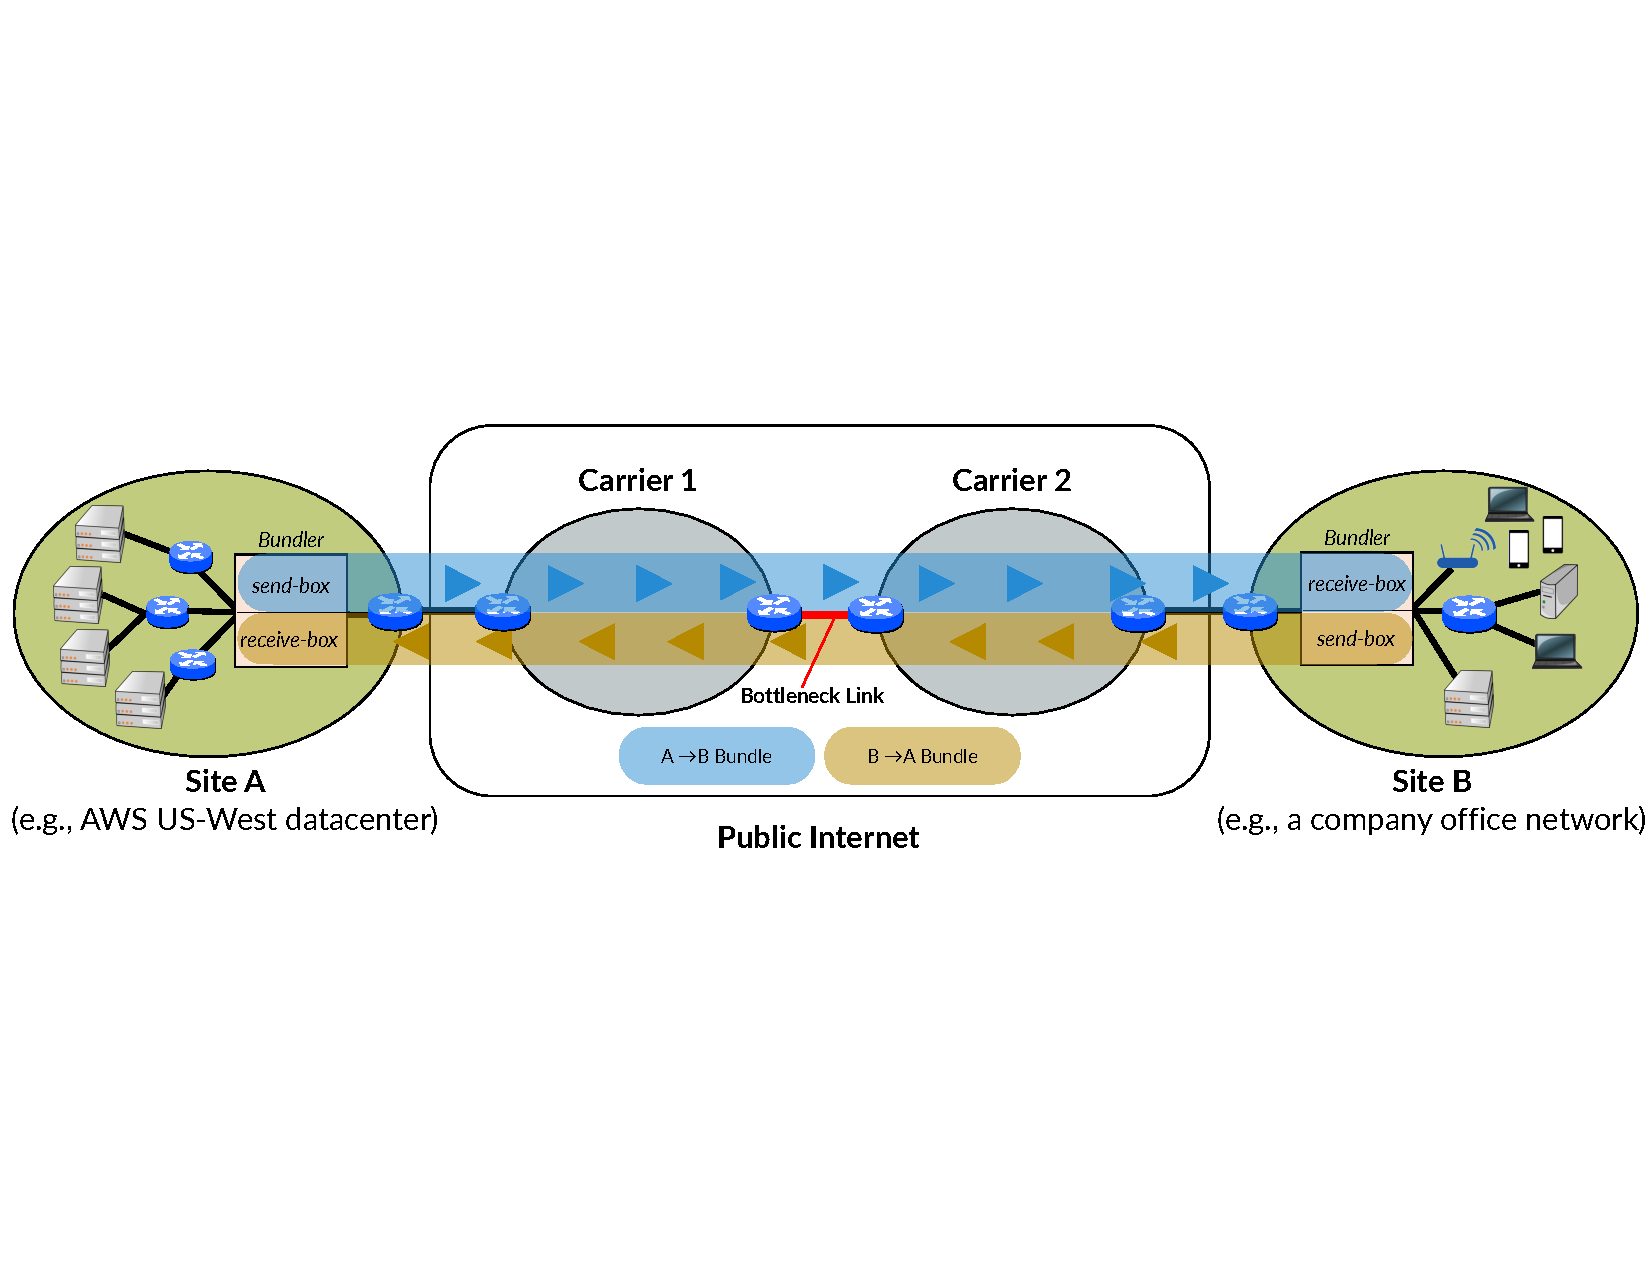
\includegraphics[width=\textwidth]{img/deployment-arch.pdf}
    \caption{An example deployment scenario for \name in sites A and B.
    Traffic between the two boxes is aggregated into a single bundle, shown as shaded boxes. The \inbox schedules the traffic within the bundle according to the policy the administrator specifies (\S\ref{s:design}).
    \an{site a and site b should be flipped}
    }
    \label{fig:deploy:arch}
\end{figure*}

%We further note that middleboxes are now prevalent in the Internet architecture~\cite{aplomb}. They are often deployed at the egress and ingress of a network domain, to ensure traffic transits them for intrusion detection, packet inspection, filtering etc. They thus provide an effective vantage point for aggregating and managing traffic. 



%Our key insight (discussed in \S\ref{s:design}) is the bundle rate control mechanism: to move the queues, we can simply use a delay-controlling congestion control algorithm. \radhika{can i chop this?}
%\an{shouldn't we keep the key insight in the intro?}

As shown in Figure~\ref{fig:deploy:arch}, \name implements its source site and destination site functions in a \emph{\inbox} and \emph{\outbox}, respectively. The \inbox of one site pairs with the \outbox of another site when sending traffic to it.\footnote{One \inbox can pair with multiple {\outbox}es and vice versa.} 
%We thus define a \emph{bundle} to be a group of flows that share the same \inbox-\outbox pair.
These two middleboxes measure congestion signals such as the round-trip time (RTT) and the rate at which packets are received, and pass these signals to a congestion control algorithm at the sendbox (\S\ref{s:design}) to dynamically compute the bundle's sending rate.
%The \inbox passes these signals to a delay-based congestion control algorithm (as described in \S\ref{s:design}) which computes appropriate sending rates for each bundle, such that the queuing induced by the bundled traffic within the network is low and is incurred at the \inbox instead, while still maintaining high utilization at the bottleneck link.
We introduce a lightweight method for the coordination between the \inbox and the \outbox that does not require any per-flow state and can be deployed in a mode that forwards packets without modification.  \name requires no changes to the end hosts or to network routers.
 
Our focus thus far has been to control traffic only within a given bundle and not across different bundles. 
Furthermore, as we will discuss in \S\ref{s:deploy}, there may be instances where \name cannot improve performance for the bundled traffic, and falls back to the status quo; \ie the performance achieved today when queues build in the network instead of the edge. For example, when traffic between the two sites traverses different paths with different levels of congestion, \name will detect this and performance will revert to the status quo.
%\cut{, but if all of these paths have the same rates, then performance will improve.\fc{<- can we cut last phrase?}}
 
In emulated scenarios (\S\ref{s:eval}), we demonstrate that \name successfully enables scheduling benefits. In particular, when configured to use Stochastic Fairness Queueing (SFQ),
\name reduces the median flow completion time (FCT) of a representative flow size distribution between 28\% to 97\% across a variety of scenarios. Furthermore, these performance benefits are within 15\% of what would be achievable if (optimal) in-network scheduling were a possibility.
In experiments over the public Internet (\S\ref{s:eval:realworld}), we find that \name reduces short-flow latencies by 57\%.

%TODO: Add evaluation highlights

\if 0
Despite these limitations, we believe that our work provides a deployable solution for enabling some of the benefits of scheduling and queue management in the Internet from the edge of the content provider's network.
 \fi
 
 \if 0
We make the following contributions:
\begin{enumerate}
    \item A light-weight, scalable, and deployable architecture that enables content providers to perform scheduling across traffic with a common destination domain. In this architecture, content providers perform congestion control over bundles of traffic with a common destination domain in order to move queueing to the content provider's edge (\S\ref{s:design}).
     \item A novel low-overhead protocol-agnostic technique for measuring signals for congestion control between the \pair, that need not make any changes to the packet headers (\S\ref{s:measurement}).
     \item A new congestion controller, synthesized from existing building blocks in congestion control (delay-control~\cite{copa}, AQM~\cite{pie}, and cross-traffic inference~\cite{nimbus} for use with traffic bundles (\S\ref{s:queue-ctl}).
     %\item The design and implementation of a \name, including a novel method of collecting congestion control information and enforcing the decisions of a rate control algorithm on traffic aggregates, which \emph{moves} the queues from the bottleneck in the network to the customer's edge.
     %\item An evaluation of the benefits of scheduling and queue management for traffic aggregates, compared to both the status quo (FIFO) and an idealized deployment where bottleneck queues deploy the desired policy.
\end{enumerate}
\fi
